\chapter{Aufbau und Konfiguration des Clusters}

Dieses Kapitel bildet die erste Hälfte des praktischen Teils der Projektarbeit.
Dieser behandelt den Aufbau der Hardware, die Netzwerk Konfiguration, sowie die Installation der Kata-Runtime und letztendlich den Aufbau eines Kubernetes Clusters.
Am Ende diese Kapitels soll alles für das sichere Deployment von Sormas auf Kata Vorbereitet sein.  

\section{Hardware}
Für das Projekt wurde folgende Hardware verwendet:
\begin{itemize}
    \item 1 Intel Atom \ac{NUC}
    \item 3 Lenovo Workstations 
    \item 1 Linksys Netzwerk-Switch
    \item 5 Ethernet Kabel
    \item 1 \ac{PDU}
    \item entsprechende \ac{PSU}s
\end{itemize}

Der einzelne Intel \ac{NUC} soll in dem Cluster die Rolle des Masters einnehmen.
Die Workstations werden als Worker eingesetzt.
Der Switch und die Ethernet Kabel werden genutzt um ein isoliertes Netzwerk aufzubauen, davon wird sich eine geringere Latenz und bessere Labor Bedingungen versprochen.
Mithilfe der \ac{PDU} und \ac{PSU}s wird das Cluster mit Strom versorgt. 
Eine Bestimmung der Hardware lässt sich Tabelle \ref{table:hardware} entnehmen, für eine detallierte Version siehe Anhang \ref{table:hw_detail}.

\begin{table}[h]
    \centering
    \begin{tabular}{ p{ 0.3\textwidth } | p{ 0.3\textwidth } p{ 0.3\textwidth } }
        x & \ac{NUC} & Workstations \\
        \hline \\
        CPU & Intel\textregistered Celeron\textregistered N2930 CPU@1.83GHz &  Intel\textregistered Core\texttrademark i3-7100 CPU@3.90GHz \\
        Cores & 4 & 4 \\
        Arbeitsspeicher & 8GB & 8GB \\
        Speicherplatz & 196GB & 240 GB \\
    \end{tabular}
    \caption{Hardware}
    \label{table:hardware}
\end{table}


\section{Vorbereitung der Maschinen}
Um die Maschinen vorzubereiten wurden bei jeder einzelnen der Storage komplett formatiert.
Anschließend wurde auf allen Maschinen Ubuntu 20.04 als \ac{OS} installiert.
Ubuntu wurde auf Empfehlungen aus dem Unternehmen gewählt, da einige schon gute Erfahrungen mit Kubernetes auf Ubuntu gesammelt haben und ein gutes Tiefewissen vorhaben ist.
\\
Für jede Maschine wurde dabei ein User und ein Passwort eingerichtet, sowie der \ac{SSH} Zugriff von Außerhalb freigeschaltet.
Der SSH-Zugriff wird benötigt um die Maschinen leichter zugänglich zu machen, aber vor allem, um Sie mit Ansibel managen zu können.


\section{Netzwerk Konfiguration}
Als nächstes muss ein Netzwerk-Zugang für die Maschinen eingerichtet werden.
Das Netzwerk soll so gut wie möglich von den Produktiv-Netzwerken bei Netzlink abgegrenzt sein.
Durch ein Subnet kann erreicht werden, dass die Netzwerk Performance erhöht wird und die Maschinen nicht von anderem Traffic beeinflusst werden können.
Dadurch können insgesamt reproduzierbarere Ergebnisse erzielt werden. 
\\
Für diese Projekt soll des Subnetz von dem Master-Node aufgespannt werden. 
Dadurch kann der Master auch an anderer Stelle einfach mit dem Netzwerk verbunden werden und das interne Netz bleibt unverändert.
Für den Master wurde also eine statische Netzlink-Interne \ac{IP}-Adresse angefragt um über diese Adresse auch die restlichen Nodes an das Netzwerk anzuschließen.
Zusätzlich erhält der Master eine interne \ac{IP}-Adresse über die er mit den Nodes kommunizieren kann.
Die gewählten Adressen lassen sich Tabelle \ref{table:katanetes_ips} entnehmmen.

\begin{table}
    \centering
    \begin{tabular}[h!]{ c | c c }
        x & Externe \ac{IP} & Interne \ac{IP} \\
        \hline
        k8smaster & 10.10.6.60 & 192.168.0.1 \\
        k8sworker1 & - & 192.168.0.11 \\
        k8sworker2 & - & 192.168.0.12 \\
        k8sworker3 & - & 192.168.0.13 \\
    \end{tabular}
    \caption{Cluster IPs}
    \label{table:katanetes_ips}
\end{table}

Das Netzwerk wurde so geplant, dass nur der Master-Node einen Internet-Zugriff beötigt.
Auf Ihm wurde ein \ac{DHCP}-Daemon so eingerichtet, dass dieser jedem der Worker basierend auf deren \ac{MAC}-Addressen die richtige IP zuordnet. 
Die Configuration für den \ac{DHCP}-Server findet sich im Anhang unter \ref{app:dhcp}. 

Um den Maschinen den Internet-Zugang zu ermöglichen muss als letztes \ac{NAT} auf dem Master Node konfiguriert werden.
Dafür muss \textbf{net.ipv4.ip\_forward=1} in die \textit{/etc/sysctl.conf} eingetragen werden und anschließend der Server rebootet.
Außerdem müssen die \textbf{iptables} Regeln angepasst werden, damit der Traffic auf dem internen Interface auf das externe Interface weitergeleitet wird. 
Das externe Interface ist das \textbf{enp4s0} und das Interne ist \textbf{enp3s0}.
Für das externe Interface, also \textbf{enp4s0} muss zunächst \textbf{POSTROUTING} und \textbf{MASQUERADE} eingerichtet werden. 
Dadurch werden die Pakete, die an diesem Interface ankommen, mit der IP des Masters maskiert und dann surch das public Interface gesendet. 

Anschließend müssen alle Pakete die an \textbf{enp3s0} geschickt werden auf \textbf{enp4s0} geforwarded werden, sowie die ankommenden Pakete auf \textbf{enp4s0} wieder über \textbf{enp3s0} zu den entsprechenden Maschienen.

Die genau Konfiguration ist im Anhang unter \ref{app:iptables} zu finden. 

In Ubuntu 20.04 wird nicht wie vielleicht bekannt mit der rc.local gearbeitet, sondern mit den Tools \textbf{iptables-persistent} und \textbf{iptables-save}.

Das entstandene Netzwerk wird in Abbildung \ref{fig:network_diagramm} dargestellt.

\begin{figure}[h]
    \centering
    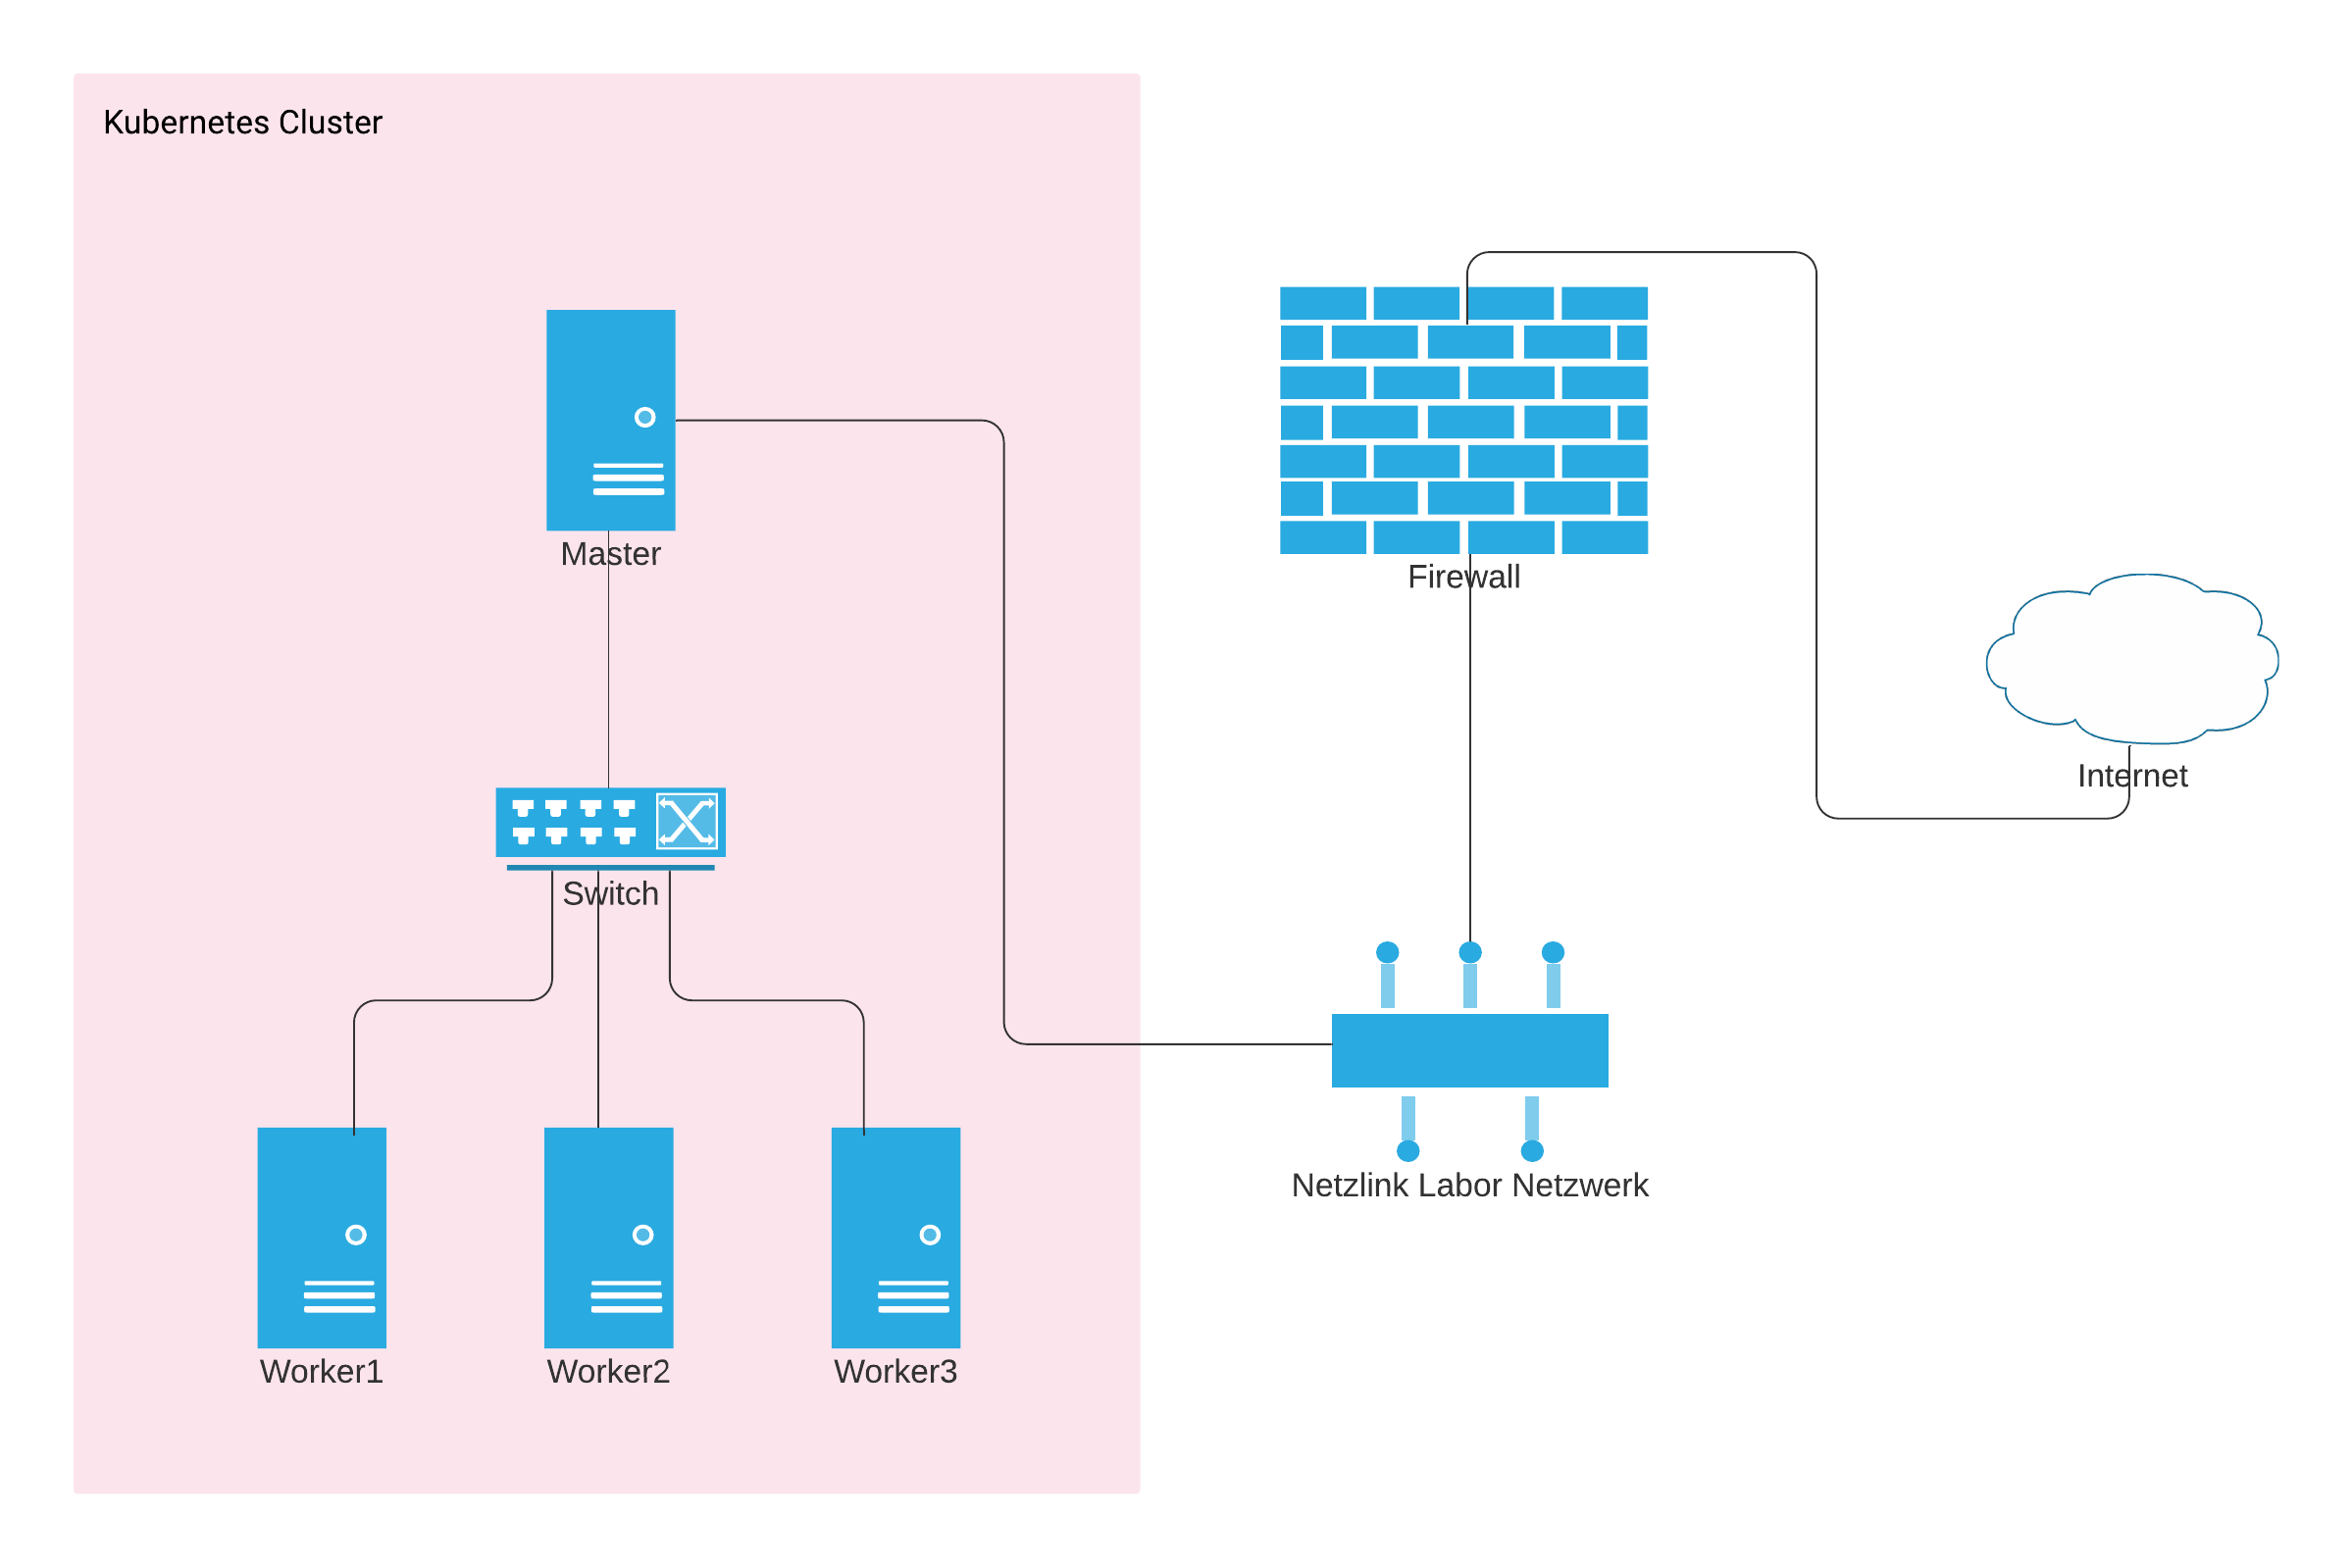
\includegraphics[width=\textwidth]{bilder/Katanetes Network.png}
    \caption{Netzwerkdiagramm}
    \label{fig:network_diagramm}
\end{figure}

\newpage

\section{Ansible Setup}
Von diesem Punkt an können nun alle Konfigurationen mit Ansible gemacht werden, da auf jeder der Maschinen \ac{SSH} konfiguriert ist und sie alle über eine Netzwerkverbindung verfügen.
Dazu muss nur auf dem Master Ansible installiert werden und der \ac{SSH} Zugang zu allen Zielsystemen konfiguriert sein. 
Für die Installation von Ansibel muss zunächst das Repository \textbf{ppa:ansible/ansible} zum Paketmanager hinzugefügt werden, dann können über \textbf{apt} die entsprechenden Pakete installiert werden.
Wie zuvor erwähnt muss die Ansibel Installation nur auf einer Maschine erfolgen.

Anschließend müssen für Ansible nur die Hosts, welche gemanaged werden sollem, in die \textit{hosts}-file eingetragen werden.
Dabei bietet Ansible die Möglichkeit Hostgruppen zu bilden. 
Wenn ein Playbok ausgeführt wird, kann die Hostgruppe angegeben werden, und alle Operationen werden dementsprechend auf alle Hosts in dieser Gruppe angewendet. 
Für dieses Projekt wurden die Gruppen \textbf{master} und \textbf{woker} gebildet.
Das Inventory kann im Anhang unter \ref{app:hosts_file} gefunden werden.

\section{Kata-Container}
\subsection{Kata Installation}

Damit Kubernetes mit Kata-Containern als Runtime aufgebaut werden kann, muss die Runtime als erstes installiert werden.
Kata benötigt eine \ac{KVM}-Software um zu funktionieren, hier wurde qemu-kvm gewählt.
Pakete die im Paket-Manger des \ac{OS} enthalten sind, können mittels des entsprechenden Ansible-Moduls installiert werden.
Für Ubuntu ist dies das \textbf{apt} Modul. 

Zur Installation von Kata wird das Tool \textbf{kata-manager}\footnote{https://github.com/kata-containers/documentation/blob/master/install/installing-with-kata-manager.md} angeboten. 
Dieses hat zwei verschiedene Installations Modi:
\begin{itemize}
    \item Full Installation \\ Hier werden die Kata-Pakete installiert, dann Docker und zuletzt wird Docker konfiguriert um standartmäßig die Kata-Runtime zu nutzen
    \item Kata packages \\ Hier werden ausschließlich die Kata-Pakete installiert
\end{itemize}
Da Kuberntes mit Containerd Installiert werden soll, wird hier auf eine zusätzliche Docker Installation verzichtet.
Um den Kata-Manager auszuführen kann einfach das Skript mit \textbf{curl} heruntergeladen werden und dann in einer Shell ausgeführt wie in \ref{lst:kata_isntall} gezeigt.
\begin{lstlisting}[language=bash, caption={Kata Installation}, label={lst:kata_isntall}]
$ bash -c "$(curl -fsSL https://raw.githubusercontent.com/kata-containers/tests/master/cmd/kata-manager/kata-manager.sh) install-packages"
\end{lstlisting}
Ansible bietet für diese Anwendungsfälle das \textbf{shell}-Modul, das auf den Zielsystemen ein Command in der Shell ausführen kann. 

Danach kann über dasselbe Modul der \textbf{kata-check} ausgeführt werden, dieser überprüft ob auf dem System nun Kata-Container ausgeführt werden können.
Nach der Überprüfung kann die Installation zunächst als erfolgreich betrachtet werden.

Allerdings wird durch das verwenden des Shell-Modules ein wichtiges Prinzip beim Entwerfen von Ansible-Playbooks verletzt. 
Diese Module werden immer ausgeführt, da sie imperativ und nicht deskriptiv sind. 
Ansible basiert aber darauf, dass Playbooks wenn möglich idempotent sein sollen.
Das beudetet, dass zunächst überprüft wird, ob der beschriebene Status bereits besteht und nur dann eine Änderung ausgeführt wird wenn dieser erst hergestellt werden muss. \cite{ansibel_idempotency}
Ein mehrfaches Auführen der Playbooks sollte keine Änderung am Endzustand bewirken, und wo möglich sollten nur beim ersten Ausführen Änderungen ausgeführt werden. 

Um diese Funktionalität auch in den imperativen Shell-Modulen abzubilden, wird zu Beginn des Playbooks überprüft, ob die Binary unter \textit{/usr/bin/kata\_runtime} bereits vorhanden ist. 
Das Ergebnis wird in einer Variabeln gespeichert, und das Shell-Modul wird nur ausgeführt wenn diese \textbf{false} ist. 

Der \textbf{kata-check} soll auf jeden Fall ausgeführt werden, da aber keine Änderungen durchgeführt werden wird \textbf{changed\_when} immer auf \textbf{false} gesetzt.

Das Playbook befindet sich auch im Anhang unter \ref{app:kata_install}.

Da hier Kubernets über \textbf{containerd} und den \textbf{contaienrd-shim-kata-v2} mit Kata kommuniziert wird in einem weiten Playbook Containerd über den Paket-Manager installiert und anschließend der Service gestartet.


\subsection{Konfiguration von Kata und Containerd}

Zur Konfiguration der beiden Programme muss jeweils eine Konfigurations-Date an der korrekten Stelle im File-System erstellt werden.
Für Kata ist die Standart-Konfiguration zunächst ausreichend. 
Um diese zu nutzen kann einfach die mitinstalliert \ac{TOML} Datei unter \textit{/usr/share/defaults/kata-containers/configuration.toml} nach \textit{/etc/kata-containers/config.toml} kopiert werden.

An der Konfiguration für \textbf{contaienrd} müssen einige Änderungen vorgenommen werden, weswegen diese Datei aus dem Ansible-Projekt nach \textit{/etc/containerd/config.toml} kopiert wird, wo diese durch einen Service restart geladen wird.
In dieser müssen die zur Verfügung stehenden Runtimes definiert werden.
Dies kann unter dem Punkt Plugins getan werden.
Dort wird der Name der Runtime definiert, über den diese später in den Manifesten referenziert werden kann.
Außerdem wird der \ac{API} Typ angegeben, sowie die Location der Konfiguration der entsprechenden Runtime.
Der wichtigste Teil der Konfiguration ist als Auszug unter \ref{lst:containerd_config} abgebildet, der Rest den Config kann im Anhang unter \ref{app:containerd_config} eingesehen werden.

\begin{lstlisting}[language=bash, caption={/etc/contaienrd/config.toml}, label={lst:containerd_config}]
[plugins]
  [plugins."io.containerd.grpc.v1.cri"]
    [plugins."io.containerd.grpc.v1.cri".containerd]
      default_runtime_name = "runc"
      [plugins."io.containerd.grpc.v1.cri".containerd.runtimes]
        [plugins."io.containerd.grpc.v1.cri".containerd.runtimes.kata]
          runtime_type = "io.containerd.kata.v2"
          privileged_without_host_devices = true
          [plugins."io.containerd.grpc.v1.cri".containerd.runtimes.kata.options]
            ConfigPath = "/etc/kata-containers/config.toml"
\end{lstlisting}

Nachdem diese Konfiguration abgeschlossen ist, ist die Kata-Runtime nicht nur installiert sondern auch für den Einsatz in Containerd und damit Kubernetes konfiguriert und einsatzbereit.


\section{Installation des Kubernetes-Clusters}

\subsection{Swap}
In der Base-Rolle werden einige Grundeinstellungen gesetzt, wie die Zeitzone etc.
Für dieses Projekt sind allerdings vor allem die Swap Einstellungen relevant, weswegen in diesem Absatz darauf eingegangen wird.
\\
Auch hier wird, um unnötige Operationen zu vermeiden, zunächst einmal überprüft, ob Swap auf der Maschine überhaupt aktiviert wird.
Wenn Swap noch nicht deaktiviert wurde wird zunächst einmal mittels des Kommandos \textbf{swapoff -a} jeder Swap ausgeschaltet.
Um diese Einstellung nach nach einem Reboot noch persistent zu haben, muss die \textit{/etc/fstab} bearbeitet werden.
Zum einheitlichen Bearbeiten von Dateien bietet Ansible das \textbf{replace}-Modul an.
Damit kann mithilfe von \ac{regex} nach bestimmen Strings gesucht werden.
Die \ac{regex} \ref{lst:regex} sucht nach allen Zeilen die "swap sw" enthalten. 
Dabei werden Leerzeichen ignoriert und nur Zeilen ausgewählt die nicht auskommentiert sind. \cite{regex}
Alle Zeilen in denen dieser Ausdruck gefunden wird, werden anschließend auskommentiert.
\begin{lstlisting}[language=bash, caption=regex, label=lst:regex]
'^([^#].*?\sswap\s+sw\s+.*)$'
\end{lstlisting}
Die Ansible-Rolle ist im Anhang unter \ref{app:base_role} zu finden.


\subsection{Installation der Kubernetes Tools}
Um die für Kubernetes benötigten Tools zu installieren wird als erstes der Verschlüsselungs-Schlüssel zum Paketmanager \textbf{apt} hinzugefügt.
Anschließend wird das Kuberntes Repository zu den \textbf{apt}-Repositorys hinzugefügt. 
Mit den Ansible Modulen \textbf{apt\_key} und \textbf{apt\_repository} lassen sich die Bedingungen leicht erfüllen.
Danach werden die benötigten Pakete installiert. 
Diese sind:
\begin{itemize}
    \item kubeadm
    \item kubectl
    \item kubelet
    \item kubernetes-cni
\end{itemize}
Die Rolle ist dem Anhang \ref{app:kube_tools} beigefügt.


\subsection{Setup des Master-Nodes}
Die folgenden Schritte werden nur auf dem Master-Node ausgeführt. 
In der Rolle wird mit dem \textbf{kubeadm} Kommando das Cluster Initialisiert.
Dabei werden folgende Argumente mitgegeben:
\begin{itemize}
    \item pod-network-cidr \\ Über dieses Argument wird das Subnetz für definiert, in welchem die Pods deployed werden können
    \item apiserver-advertise-address \\ Die \ac{IP} Adresse auf welcher der \ac{API}-Server aufgesetzt werden soll
    \item apiserver-cert-extra-sans \\ Zusätzliche Domain Names und \ac{IP} Addressen, die in das Zertifikat für den \ac{API}-Server eingebunden werden sollen
    \item token-ttl \\ Die \ac{TTL} die ein Token hat, bevor er abläuft
    \item token \\ Der Token mit dem sich die Worker an dem Kubernetes Cluster anmelden können. Eigentlich würde Kubernetes einen eigenen Token generieren, hier muss jedoch ein statischer gesetzt werden, damit er im nächsten Schritt, dem Join der Worker, verwendet werden kann
\end{itemize}
Das vollständige Kommando ist als \ref{lst:init} angegeben.
\begin{lstlisting}[language=bash, caption={kubeadm init}, label=lst:init]
/usr/bin/kubeadm init \
--pod-network-cidr 10.244.0.0/16 \
--apiserver-advertise-address 192.168.0.1 \
--apiserver-cert-extra-sans "katanetes.netzlink.com,k8smaster,10.10.6.60,192.168.0.1,api.katernetes.local" \
--token-ttl 24h0m0s \
--token ad623b.c501de9c4fab8e7f
\end{lstlisting}

Danach wird noch die \textit{.kube/config} in das Home-Verzeichnis des Users kopiert und mit den richtigen Rechten versehen, damit dieser das Cluster managen kann.
Die Rolle ist dem Anhang unter \ref{app:master_setup} beigefügt.

Zu Beginn des Playbooks wird überprüft ob eine kubelet Configuration bereits vorhanden ist. 
Ist dies der Fall wird Kubernetes zunächst resettet um anschließend eine funktionierende Version ausrollen zu können.
Die entsprechende Rolle ist dem Anhang unter \ref{app:reset} beigefügt.


\subsection{Join der Worker}
Auch in dieser Rolle wird zunächst überprüft ob schon eine \textit{kubelet.conf} existiert, und der Zustand entsprechend zurückgesetzt, wenn dies zutrifft.
Danach wird noch einmal überprüft ob IPv4 Forwarding korrekt konfiguriert ist, da diese Einstellungen durch das \textbf{kubeadm\ reset} beeinflusst werden könnten.
Das eignetliche Join der Nodes ist ein einfaches Shell-Command, dem als Arguemnt der Token übergeben werden kann, der im vorheringen Absatz statisch gesetzt wurde.
Die Rolle ist im Anhang unter \ref{app:join_role}


\subsection{Weitere Konfigurationen}
An diesem Punkt steht das komplette Kubernetes Cluster.
Um einen vollen Funktionsumfang zu ermöglichen müssen allerdings noch einige Anwendungen auf dem Cluster deployed werden.

\subsubsection{Networking}
Damit die Pods untereinander kommunizieren können, muss ein Container Network aufgesetzt werden.
In der Firma wurde hier Calico empfolen, dieses \ac{CNI} konnte allerdings auch nach ausgiebigem Testen nicht erflgreich mit Kata eingesetzt werden.
Obwohl eigentlich eine Untersützung auf der Website dokumentiert wurde, konnten die Container, welche in der Kata-Runtime liefenn, nicht miteinander kommunizieren.
Als Alternative wurde dann die Empfehlung von Kata befolgt, und zu Flannel\footnote{https://github.com/coreos/flannel} gewechselt. 
Mit diesem \ac{CNI} wurden alle Netzwekprobleme, die zuvor bestanden behoben.
\\
Das Netzwerk kann mittels \textbf{kubectl apply} ausgerollt werden.
Damit das Deployment durchgeführt werden kann, muss Ansible an dieser Stelle von dem Root User zu dem Alberto-User wechseln, da nur für ihn die Kube-Config eingerichtet ist. \todo{Alberto früher erwähnen}

\subsubsection{Ingress}
Für Ingress wurde zunächst auf Empfehlung von Kollegen traeffik getestet. 
Hierbei ergaben sich einige Probleme mit der Terminierung von \ac{TLS}, weswegen letztendlich zu dem Standart NGINX gewechselt wurde.

In einer traditionellen Cloud Umgebung werden vom Cloud Anbieter auch Load Balancer zur Verfügung gestellt. 
Diese bieten einen "single point of contact" für den Ingress, alle Anfragen werden von dem Load Balancer an die Ingress Controller verteilt und diese Verteilen an die einzelnen Applikationen weiter.
In diesem Projekt ist das Cluster aber nicht in einer Cloud-Umgebung gehostet sondern auf bare metal.
Es steht kein externer Load-Balancer zur Verfügung und so muss an anderer Weg gefunden werden um denn Ingress Controller zum Einsatz zu bringen. 

Um trotzdem aus dem Netzwerk auf den Ingress Controller zugreifen zu können, wird dem Service eine externe ClusterIP zugewiesen.
Der Traffic, der auf dieser \ac{IP} ankommt, wird dann zu einem der Service-Endpoints geroutet.
Als externe \ac{IP} wird die Addresse das Master-Nodes eingetragen, sowie die \ac{HTTP} und \ac{HTTPS} Ports 80 und 443.
Durch diese Configuration werden alle Anfragen, die an den Hostnamen des Masters geschickt werden, an dem Ingress Controller Service ankommen, von wo aus sie an den Ingress Pod geschickt werden.
\\
Der Ingress selbst ist dann dafür zuständig anhand der prefixe der Addressen die Anfragen an die richtigen Services weiterzuleiten.
Diese Architektur ist in Abbildung \ref{fig:clusterip} dargestellt.
\begin{figure}[h!]
    \centering
    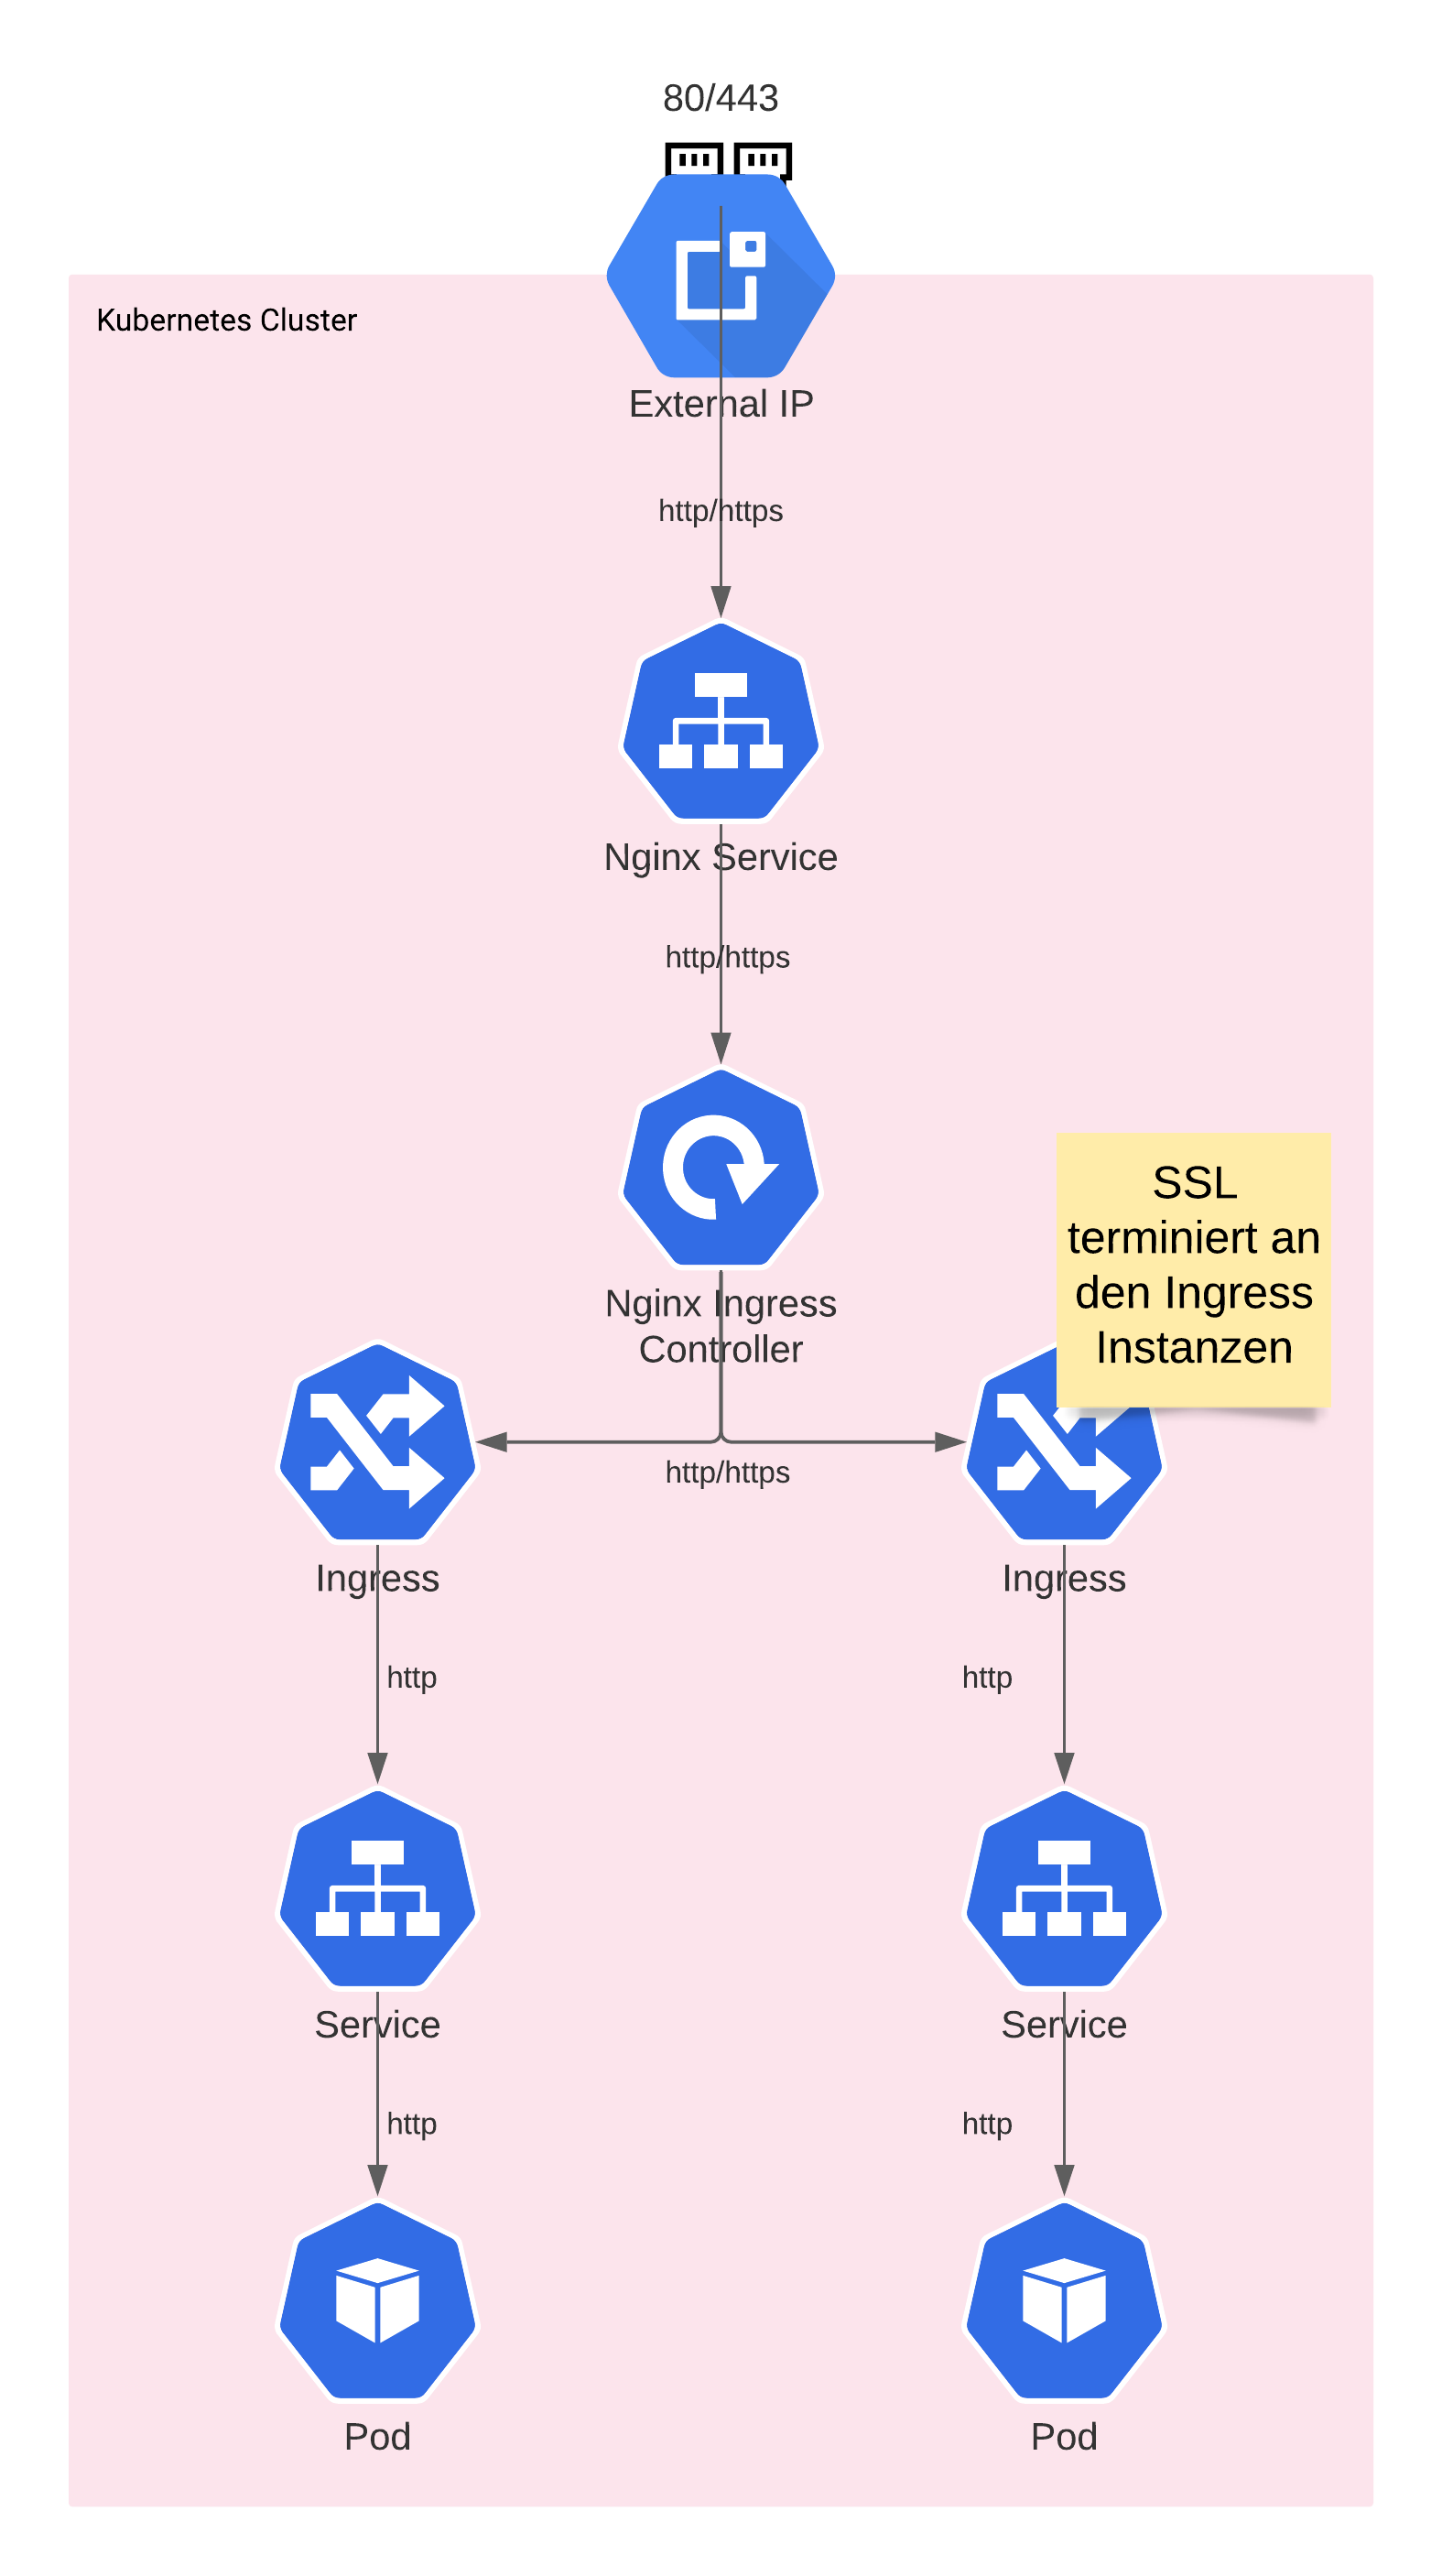
\includegraphics[width=0.8\textwidth]{bilder/ClusterIP.png}
    \caption{Ingress Cluster IP Architektur}
    \label{fig:clusterip}
\end{figure}
Zum Deployment des Ingress wurde die Standart-Anleitung\footnote{https://github.com/nginxinc/kubernetes-ingress} verwendet.
Die einzige Änderung ist hier das Umändern des Service Typen zu einer externalIP und das Freigeben der entsprechenden Ports.
Diese Änderungen sind dem Anhang unter \ref{app:clusterip} beigefügt.
\\
Das Deployment wird über Ansible gemanaged, in dem Playbook werden die nötigen \ac{YAML} Konfigurations Dateine auf den Master kopiert und dann mittels \textbf{kubctl apply} angewandt. 


\subsubsection{Storage}
Um mit \ac{PV}s arbeiten zu können muss dafür ein Provider vorhanden sein, der den angefragten Block Storage zur Verfügung stellen kann. 
In den Cloud Umgebungen wird das, wie auch die Load Balancer, von dem Cloud Provider gemanaged. 
Auf der bare metal Lösung muss dies eigenständig getan werden, mit Software-Lösungen wie Longhorn.\footnote{https://longhorn.io}
Longhorn erstellt für jedes Volume einen dedizierten Storagfe Controller und repliziert das Volume über verschiedene Nodes.
Damit wird die Persistenz gewährleistet.
Durch ein DaemonSet wird auf jedem Node ein Manager Pod gehostet, der für das erstellen und managen von den Volumes der Nodes zuständig ist. 
\\
Longhorn wird über \textbf{helm} installiert. 
Um Helm zu installieren wird zunächst die Installationsanleitung\footnote{https://helm.sh/docs/intro/install/} in Ansible abgebildet.
Diese beinhaltet das Hinzufügen der Verschlüsselungs Keys und des helm-Repositorys zu \textbf{apt}, das Installieren des \textbf{apt-transport-https} Pakets, und schließlich das Installieren des Helm Pakets.
\\
Wenn das Helm Paket installiert ist wird das Longhorn Repository über das \textbf{git} Modul hinzugefügt, ein Namespace für longhorn angelegt und dann Longhorn deloyed.
Die komplette Rolle ist dem Anhang unter \ref{app:longhorn} beigefügt.

\subsubsection{Dashboard}
Die letzte Funktionalität, die für ein vollwertiges Kubernetes-Cluster noch fehlt, ist eine Möglichkeit, die Pods in irgendeiner weise zu monitoren.
Das Kubernetes Dashboard bietet simple Monitoring-Funktionen sowie die Möglichkeit Änderungen durchzuführen, Ressourcen zu löschen, erstellen und einzusehen.
Um das Dashboard zu installieren wurde mit der aktuellen Installationsanleitung\footnote{https://kubernetes.io/docs/tasks/access-application-cluster/web-ui-dashboard/} von Kubernetes gearbeitet.
Zum Zugriff auf das Dashbaord muss User und ein ClusterRoleBinding erstellt werden. 
Mit dem Token dieses Users kann sich dann an dem Dashboard angemeldet werden, um dieses sinnvoll nutzen zu können.\footnote{https://github.com/kubernetes/dashboard/blob/master/docs/user/access-control/creating-sample-user.md}

\todo{monospaceschriftart}
